\documentclass[10pt]{article}

\newlength\tindent
\setlength{\tindent}{\parindent}
\setlength{\parindent}{0pt}
\renewcommand{\indent}{\hspace*{\tindent}}
\pagestyle{empty}

\usepackage{graphicx}
% \usepackage{times}
\usepackage{ebgaramond}
\renewcommand{\familydefault}{\sfdefault}

\usepackage{geometry}
\geometry{ansiapaper, margin=0.75in, top=0.7in}
\usepackage{tikz}
\usetikzlibrary{calc}

\setlength\parindent{0mm}

\usepackage{wasysym}
\usepackage{marvosym}
\usepackage{fontawesome5}

\renewcommand{\section}[4]{%
  \medskip
  
  \begin{tikzpicture}
    \node (#1) [rectangle, minimum width=1.0\linewidth, 
    anchor=north west,
    shading = radial, % shading angle=135,
    outer color=#4!80,inner color=white
    % axis left color=#3,
    % middle color = white,
    % right color = #4
    ]
    at (0pt, 0pt) {
      \textbf{\Large #2}
    };
  \end{tikzpicture}
}

\definecolor{colorsection}{HTML}{7393B3}
\newcommand{\mynewsection}[2]{%
  \medskip

  \textbf{\color{colorsection}\LARGE {#2}\hspace{0.25in}{#1}}
}


\renewcommand{\subsection}[1]{%

  \medskip
  
  %\noskill
}

% \definecolor{left} {HTML}{AFE1AF}
% \definecolor{right} {HTML}{50C878}

\usepackage{hyperref}
\hypersetup{
  colorlinks=true,
  linkcolor=darkblue,
  filecolor=magenta,      
  urlcolor=cyan,
  pdftitle={Serge CHASTEL - Resume - 2021-09-03},
}
  
\begin{document}

{ \Large \textbf{Serge CHASTEL, PhD} Software/Data Engineer }

\medskip
        
17+ years of experience designing, developing, integrating, and
deploying cutting-edge engineering solutions based on distributed
computing and distributed storage in research institutions and
high-tech industries

\Mobilefone{}
+1 (808) 277-5687
\hfill
\Email{}
\href{mailto:schastel.at.work@gmail.com}{schastel.at.work@gmail.com}
\hfill
\faIcon{linkedin}
\href{https://www.linkedin.com/in/serge-chastel-76aa46218/}{LinkedIn}
\hfill
\Letter{}
\begin{tabular}[t]{l}
  2063 St Louis Dr. \\
  Honolulu HI, 96816
\end{tabular}

\mynewsection{Skills}{\faTasks}

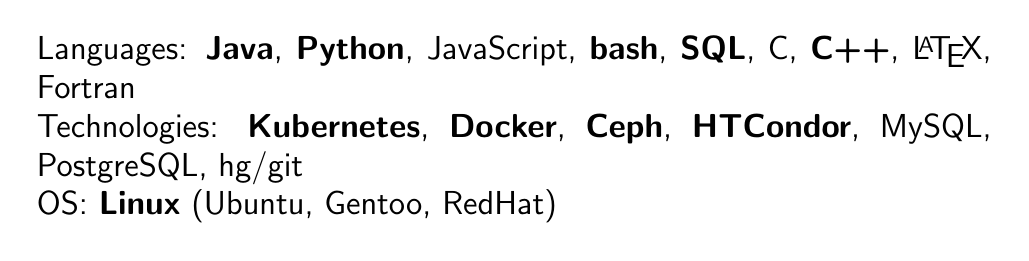
\begin{tikzpicture}
  \node [rectangle, minimum width=\linewidth,
  anchor=north west] {
    \begin{minipage}{1.0\linewidth}
      \large Languages: \textbf{Java}, \textbf{Python}, JavaScript,
      \textbf{bash}, \textbf{SQL}, C, \textbf{C++}, \LaTeX{}, Fortran

      Technologies: \textbf{Kubernetes}, \textbf{Docker},
      \textbf{Ceph}, \textbf{HTCondor}, MySQL, PostgreSQL, hg/git

      OS: \textbf{Linux} (Ubuntu, Gentoo, RedHat)
    \end{minipage}
  };
\end{tikzpicture}

\mynewsection{Experience}{\faBriefcase}

\newlength{\expitem}
\setlength{\expitem}{0.60\linewidth}

\newlength{\expskill}
\setlength{\expskill}{0.39\linewidth}

\newlength{\itemskilljump}
\setlength{\itemskilljump}{0mm}

% \experience{}{%
% }{%
% }{%
% }{%
% }
\newcommand{\experience}[5]{%
  \node (origin) [rectangle, minimum width=1.0\linewidth,
  anchor=south west,
  inner ysep = 2pt,
  shading = axis, shading angle=0,
  left color=colorsection!30!white,
  right color = colorsection!10!white] {%
    \hspace*{-7mm}
    \begin{minipage}{0.95\linewidth}
      \medskip
        
      \textbf{\large #1}
      \hfill
      \textit{\small #2}

      {\small #4}
      \hfill    
      \textit{\small #3}

      \textbf{#5}
    \end{minipage}
  };
}

\begin{tikzpicture}
  \experience{Software and Data Engineer}{%
    \href{https://neo.ifa.hawaii.edu/}{Pan-STARRS Telescopes - Moving
      Objects Processing System (MOPS)}}{%
    \href{https://www.rcuh.com/}{Research Corp. of Univ. of Hawai`i} / \href{https://www.ifa.hawaii.edu/}{Inst. for Astronomy} / \href{https://www.nasa.gov/}{NASA}}{%
    Since Mar 2013 --- 8.5 years}{%
    Specification, migration, rationalization, improvement, expansion,
    and maintenance of the MOPS}

  \node (item1) [rectangle, minimum width=\linewidth,
  anchor=north west] at ([xshift=\itemskilljump, yshift=-\itemskilljump]origin.south west) {
    \begin{minipage}{1.0\linewidth}
      \textit{Objective:} Find all asteroids/comets larger than 140m
      coming near the Earth.
      
      \textit{Challenge:} 600 observations/night ( = 4TB/night). ETL
      them so that new asteroids can quickly be followed up by other
      telescopes around the globe. The MOPS must be running 24/7,
      365/yr.

      \textit{2013:} Processing started at 8am, finished at 6pm

      \textit{2021:} Stream-based processing that starts with the
      first observation and finishes at 7am

      Software samples:
      \faIcon{github}\href{https://github.com/psmops}{github.com/psmops}
      (unfortunately not all of it since some of it is proprietary)
    \end{minipage}
  };

  \node (item2) [rectangle, minimum width=\linewidth,
  anchor=north west] at ([xshift=\itemskilljump, yshift=-\itemskilljump]item1.south west) {
    \begin{minipage}{1.0\linewidth}
      \textbf{Scientific Workflow Design and Development}: Performance
      can only be achieved through automation. The existing 2013
      system required many blocking manual human interventions and was
      replaced by a fully automated one. I also moved the HTCondor
      based distributed computing to Kubernetes using Docker

      \hfill\textbf{Kubernetes}, \textbf{Ceph}, \textbf{Docker}, HTCondor,
      MySQL, PostgreSQL, Java, JPA/Hibernate, bash
    \end{minipage}
  };
  
  \node (item3) [rectangle, minimum width=\linewidth,
  anchor=north west] at ([xshift=\itemskilljump, yshift=-\itemskilljump]item2.south west) {
    \begin{minipage}{1.0\linewidth}
      \textbf{Integration, parallelization, and distribution}: of data
      processing functions: Scientists write software and are
      oblivious of system constraints. I was in charge of their
      integration in the system. Constraints related to the
      parallelization and distribution forced sometimes full rewrites
      of the initial code.

      \hfill\textbf{Java}, \textbf{C++}, \textbf{Python}, C, R, Fortran, IDL
    \end{minipage}
  };

  \node (item4) [rectangle, minimum width=\linewidth,
  anchor=north west] at ([xshift=\itemskilljump, yshift=-\itemskilljump]item3.south west) {
    \begin{minipage}{1.0\linewidth}
      \textbf{Definition and rationalization} of the hardware
      computing and storage medium-size HPC infrastructure. Migration
      between two sites (while keeping it up). Purchase, installation,
      deployment: \$20k/yr; 15 nodes / 544 CPUs / 4 TiB RAM / 500 TB
      storage.

      \hfill\textbf{Linux/Ubuntu}, Gentoo, \textbf{Kubernetes},
      \textbf{cephfs}, ganglia, nagios...
    \end{minipage}
  };

  \node (item5) [rectangle, minimum width=\linewidth,
  anchor=north west] at ([xshift=\itemskilljump, yshift=-\itemskilljump]item4.south west) {
    \begin{minipage}{1.0\linewidth}
      \textbf{Software Stack Code Management and Documentation}  

      \hfill\textbf{CI} through Github actions, \textbf{git}, hg, subversion,
      \textbf{Jira}, \textbf{Confluence}
    \end{minipage}
  };

  \node (item6) [rectangle, minimum width=\linewidth,
  anchor=north west] at ([xshift=\itemskilljump, yshift=-\itemskilljump]item5.south west) {
    \begin{minipage}{1.0\linewidth}
      \textbf{GUI Design and Development}: The astronomers required a
      reactive interface to monitor and vet the processing products.

      \hfill\textbf{Java} (Javalin, Apache Velocity), \textbf{Javascript}, Perl/Mason 
    \end{minipage}
  };

  \node (item7) [rectangle, minimum width=\linewidth,
  anchor=north west] at ([xshift=\itemskilljump, yshift=-\itemskilljump]item6.south west) {
    \begin{minipage}{1.0\linewidth}
      \textbf{Outreach} support for researchers, students, and
      \href{http://iasc.cosmosearch.org/}{dedicated outreach program}
    \end{minipage}
  };

  \node (item8) [rectangle, minimum width=\linewidth,
  anchor=north west] at ([xshift=\itemskilljump, yshift=-\itemskilljump]item7.south west) {
    \begin{minipage}{1.0\linewidth}
      Since May 2020 (1.5 year) \textbf{Technical Expert} for the Minor Planet Center Users Group (Small
      Bodies Node/NASA)
    \end{minipage}
  };
\end{tikzpicture}

\begin{tikzpicture}
  \experience{System Administrator/Front-End Software Engineer}{%
    Pan-STARRS 1 Telescope / Image Proc. Pipeline}{%
    Researcher Corp. of Univ. of Hawai`i / Institute for Astronomy}{%
    Jun 2010 - Feb 2013 --- 2.75 years}{%
    Hardware resources administration and front-end activities}

  \node (item1) [rectangle, minimum width=\linewidth,
  anchor=north west] at ([xshift=\itemskilljump, yshift=-\itemskilljump]origin.south west) {
    \begin{minipage}{1.0\linewidth}
      \textbf{MySQL} servers administration and optimization; HTTP
      Server administration; Cluster administration; Monitoring

      \hfill{}MySQL, bash, C, Perl, \textbf{Python}, Apache HTTP; NFS;
      Ganglia; Nagios.
    \end{minipage}
  };

  \node (item2) [rectangle, minimum width=\expitem,
  anchor=north west] at ([xshift=\itemskilljump, yshift=-\itemskilljump]item1.south west) {
    \begin{minipage}{\linewidth}
      Liaison between subsystems: Interface definition,
      requirements, and implementation
      \hfill{}PHP, HTML, CSS, \textbf{JavaScript}
    \end{minipage}
  };
\end{tikzpicture}

\begin{tikzpicture}
  \experience{Integration Software Engineer/Contractor}{%
    Atos Origin (Toulouse, France)}{%
    Customer: European Space Agency (GAIA Project)}{%
    Mar 2008 - Apr 2010 --- 2 years}{%
    Standardization and integration of scientific computing software
    modules}
  
  \node (item1) [rectangle, minimum width=1.0\linewidth, anchor=north west]
  at ([xshift=\itemskilljump, yshift=-\itemskilljump]origin.south
  west) {
    \begin{minipage}{1.0\linewidth}
      Responsible for software integration and documentation
      activities for producing an integrated scientific computing
      framework based on \textbf{machine learning techniques}\hfill
      \textbf{Java},~\textbf{JUnit},~weka~(ML~Java)
    \end{minipage}
  };
  
  \node (item2) [rectangle, minimum width=1.0\linewidth, anchor=north west]
  at ([xshift=\itemskilljump, yshift=-\itemskilljump]item1.south
  west) {
    \begin{minipage}{1.0\linewidth}
      Design and implementation of an original automated code
      generation framework for the execution of \textbf{scientific
        workflows} on a Torque/Maui-based cluster.
      \hfill UML, \textbf{Java}, ant, \textbf{Torque/Maui}
    \end{minipage}
  };

  \node (item3) [rectangle, minimum width=1.0\linewidth, anchor=north west]
  at ([xshift=\itemskilljump, yshift=-\itemskilljump]item2.south
  west) {
    \begin{minipage}{1.0\linewidth}
      \textbf{Liaison} for teams of scientists at participating
      European partner universities (UK, Germany, Spain, Italy,
      Greece, France, Belgium) to see their code tested and integrated
      into the scientific workflows

      \textbf{Liaison} between scientific teams and ESA
      industrialization partners
      \hfill JNI, SVN, Wiki, \LaTeX{}, Mantis, XML/XSLT
    \end{minipage}
  };
\end{tikzpicture}

\begin{tikzpicture}
  \experience{Test Software Engineer / Contractor}{%
    CRIL Technology/Alyotech (Toulouse, France)}{%
    Customer: \href{https://en.wikipedia.org/wiki/Astrium}{EADS Astrium}}{%
    Aug 2006 - Feb 2008 --- 1.5 years}{%
    Design, development, and in situ use of benchmarks for
    earth-observation instruments}

  \node (item1) [rectangle, minimum width=1.0\linewidth, anchor=north west]
  at ([xshift=\itemskilljump, yshift=-\itemskilljump]origin.south
  west) {
    \begin{minipage}{1.0\linewidth}
      \textbf{Requirement analysis}, \textbf{specification},
      \textbf{design}, and \textbf{development} of a generic benchmark
      for testing and validation of Earth observation optical
      instruments

      \hfill UML, \textbf{Java}, \textbf{Python}, XML/XSD,
      PV-Wave/Jwave (Fortran), IBM Rationale (ClearCase, ClearQuest),

      \hfill MS Windows 2003, XP32, XP64

      \textbf{Technical and commercial support} for software
      development activities at CRIL/Alyotech
    \end{minipage}
  };
\end{tikzpicture}

\begin{tikzpicture}
  \experience{Test Software Engineer  / Contractor}{%
    CRIL Technology (Toulouse, France)}{%
    Customer: French Civil Air Navigation Control Agency (DSNA)}{%
    Mar 2005 - Jul 2006 --- 1.25 years}{%
    Development and integration of stubs for air traffic control}

  \node (item1) [rectangle, minimum width=1.0\linewidth, anchor=north west]
  at ([xshift=\itemskilljump, yshift=-\itemskilljump]origin.south
  west) {
    \begin{minipage}{1.0\linewidth}
      Development, testing, and documentation of stubs for aerial
      control software stack

      \hfill UML, \textbf{C++}, libxml2, ACE, Corba, \textbf{rpmbuild}, \textbf{Linux} (RHEL)
      
      System maintenance of Unix servers
      \hfill\textbf{Unix} (Solaris, AIX, HP-UX)
    \end{minipage}
  };
\end{tikzpicture}

\begin{tikzpicture}
  \experience{Software Developer  / Freelance}{%
    eEyeCare GmbH (Erlangen, Germany)}{%
    }{%
    Mar 2004 - Nov 2004 --- 0.75 years}{%
    Research and Development of a tool for retinal images analysis}

  \node (item1) [rectangle, minimum width=1.0\linewidth, anchor=north west]
  at ([xshift=\itemskilljump, yshift=-\itemskilljump]origin.south
  west) {
    \begin{minipage}{1.0\linewidth}
      Quantitative performance analysis (algorithmic complexities,
      comparison of various implemented methods, experimental
      validation against ground truth)      
      \hfill UML, Design Patterns, \textbf{C++}, Java (MMI), XML
    \end{minipage}
  };
\end{tikzpicture}

\begin{tikzpicture}
  \experience{Teaching}{%
    USA, France, Germany}{%
    }{%
    18 semesters total}{%
    All teaching activities were at the undergraduate level
  \hfill Details in \href{https://www.linkedin.com/in/serge-chastel-76aa46218}{LinkedIn}}

  % \node (origin) [rectangle, minimum width=\linewidth,
  % anchor=south west,
  %   shading = axis, shading angle=135,
  %   left color=left!20!white,
  %   right color = right!20!white] {
  %   \begin{minipage}{0.95\linewidth}
  %     \subsection{Teaching}
  %     \hfill
  %     18 semesters total
      
  %     All teaching activities were at the undergraduate level
  %   \end{minipage}
  % };

  % \node (item1) [rectangle, minimum width=\expitem, anchor=north west]
  % at ([xshift=\itemskilljump, yshift=-\itemskilljump]origin.south
  % west) {
  %   \begin{minipage}{\expitem}
  %     Adjunct Professor  \hfill University of Hawai`i

  %     2015-2016 (3 semesters)
  %   \end{minipage}
  % };
  % \node (skill1) [rectangle, minimum width=\expskill,
  % anchor=north west] at ([xshift=\itemskilljump]item1.north east) {
  %   \begin{minipage}{\expskill}
  %     Operating Systems
  %   \end{minipage}
  % };
    
  
  % \node (item2) [rectangle, minimum width=\expitem, anchor=north west]
  % at ([xshift=\itemskilljump, yshift=-\itemskilljump]item1.south
  % west) {
  %   \begin{minipage}{\expitem}
  %     Invited Lecturer \hfill University of Koblenz-Landau (Koblenz, Germany)

  %     2002-2004 (3 semesters)
  %   \end{minipage}
  % };
  % \node (skill2) [rectangle, minimum width=\expskill,
  % anchor=west] at ([xshift=\itemskilljump]item2.east) {
  %   \begin{minipage}{\expskill}
  %     Digital Image Databases
      
  %     Geometry for Digital Imaging

  %     Introduction to C++
  %   \end{minipage}
  % };
  
  % \node (skill3) [rectangle, minimum width=\expskill,
  % anchor=north west] at ([xshift=\itemskilljump]skill2.south west) {
  %   \begin{minipage}{\expskill}
  %     Calculus, Algebra

  %     Statistics

  %     C programming

  %     Introduction to graph theory
  %   \end{minipage}
  % };
  % \node (item3) [rectangle, minimum width=\expitem, anchor=north east]
  % at ([xshift=\itemskilljump, yshift=-\itemskilljump]skill3.north
  % west) {
  %   \begin{minipage}{\expitem}
  %     Teaching Assistant then Adjunct Professor \hfill University of Saint-Étienne

  %     1997-2002 (12 semesters) \hfill (Saint-Étienne, France)
  %   \end{minipage}
  % };
\end{tikzpicture}


\mynewsection{Education}{\faGraduationCap}
% \definecolor{leftedu} {HTML}{87CEEB}
% \definecolor{rightedu} {HTML}{B6D0E2}
% \section{edu}{Education}{leftedu}{rightedu}

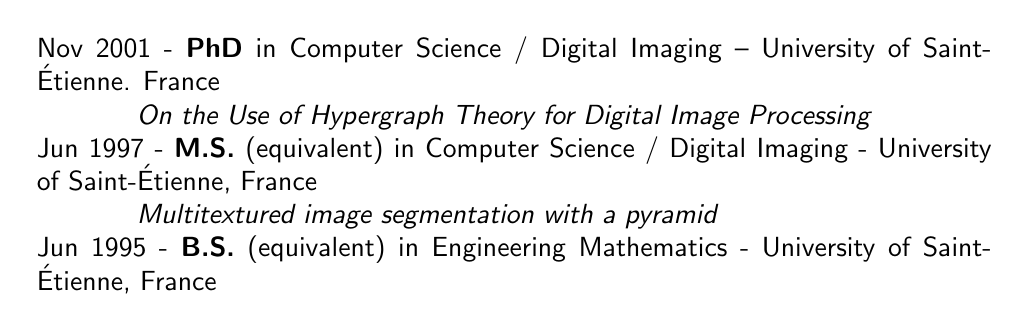
\begin{tikzpicture}
  \node (origin) [rectangle, minimum width=\linewidth,
  anchor=south west] {
    \begin{minipage}{1.0\linewidth}
      Nov 2001 - \textbf{PhD} in Computer Science / Digital Imaging –
      University of Saint-Étienne. France

      \hspace*{.5in}\emph{On the Use of Hypergraph Theory for Digital Image Processing}

      Jun 1997 - \textbf{M.S.} (equivalent) in Computer Science /
      Digital Imaging - University of Saint-Étienne, France

      \hspace*{.5in}\emph{Multitextured image segmentation with a pyramid}

      Jun 1995 - \textbf{B.S.} (equivalent) in Engineering Mathematics -
      University of Saint-Étienne, France
    \end{minipage}
  };
\end{tikzpicture}

\mynewsection{Miscellaneous}{\faBookmark}

Languages: French (native), German (Written and oral comprehension)

\emph{I'm not sure if I really qualify as a scholar
  (\href{https://scholar.google.com/citations?user=Dw3bjDYAAAAJ&hl=en}{Google})
  or a researcher
  (\href{https://www.researchgate.net/profile/Serge-Chastel}{ResearchGate})
  but I take pride in thinking that the software and the system I
  develop seems useful enough to grant me a co-authorship in many
  high-level scientific publications. e.g.:} for the
\href{https://en.wikipedia.org/wiki/\%CA\%BBOumuamua}{first
  interstellar object ever observed}, the article in
\href{https://www.nature.com/articles/nature25020}{Nature}.

\end{document}
